\documentclass[10pt]{beamer}\usepackage[]{graphicx}\usepackage[]{color}
%% maxwidth is the original width if it is less than linewidth
%% otherwise use linewidth (to make sure the graphics do not exceed the margin)
\makeatletter
\def\maxwidth{ %
  \ifdim\Gin@nat@width>\linewidth
    \linewidth
  \else
    \Gin@nat@width
  \fi
}
\makeatother

\definecolor{fgcolor}{rgb}{0.345, 0.345, 0.345}
\newcommand{\hlnum}[1]{\textcolor[rgb]{0.686,0.059,0.569}{#1}}%
\newcommand{\hlstr}[1]{\textcolor[rgb]{0.192,0.494,0.8}{#1}}%
\newcommand{\hlcom}[1]{\textcolor[rgb]{0.678,0.584,0.686}{\textit{#1}}}%
\newcommand{\hlopt}[1]{\textcolor[rgb]{0,0,0}{#1}}%
\newcommand{\hlstd}[1]{\textcolor[rgb]{0.345,0.345,0.345}{#1}}%
\newcommand{\hlkwa}[1]{\textcolor[rgb]{0.161,0.373,0.58}{\textbf{#1}}}%
\newcommand{\hlkwb}[1]{\textcolor[rgb]{0.69,0.353,0.396}{#1}}%
\newcommand{\hlkwc}[1]{\textcolor[rgb]{0.333,0.667,0.333}{#1}}%
\newcommand{\hlkwd}[1]{\textcolor[rgb]{0.737,0.353,0.396}{\textbf{#1}}}%

\usepackage{framed}
\makeatletter
\newenvironment{kframe}{%
 \def\at@end@of@kframe{}%
 \ifinner\ifhmode%
  \def\at@end@of@kframe{\end{minipage}}%
  \begin{minipage}{\columnwidth}%
 \fi\fi%
 \def\FrameCommand##1{\hskip\@totalleftmargin \hskip-\fboxsep
 \colorbox{shadecolor}{##1}\hskip-\fboxsep
     % There is no \\@totalrightmargin, so:
     \hskip-\linewidth \hskip-\@totalleftmargin \hskip\columnwidth}%
 \MakeFramed {\advance\hsize-\width
   \@totalleftmargin\z@ \linewidth\hsize
   \@setminipage}}%
 {\par\unskip\endMakeFramed%
 \at@end@of@kframe}
\makeatother

\definecolor{shadecolor}{rgb}{.97, .97, .97}
\definecolor{messagecolor}{rgb}{0, 0, 0}
\definecolor{warningcolor}{rgb}{1, 0, 1}
\definecolor{errorcolor}{rgb}{1, 0, 0}
\newenvironment{knitrout}{}{} % an empty environment to be redefined in TeX

\usepackage{alltt}
\usetheme{Warsaw}
\usepackage{graphicx}
\usepackage{amsfonts}
\usepackage{indentfirst}
\usepackage{amsmath}
\usepackage[polish]{babel}
\usepackage{polski}
\usepackage[utf8]{inputenc}
\usepackage{natbib}


\usepackage{tikz}
\usepackage{ifthen}
\usepackage{xxcolor}
\usetikzlibrary{arrows}
\usetikzlibrary[topaths]
\usetikzlibrary{decorations.pathreplacing}
%\usepackage{times}\usefonttheme{professionalfonts}  % times is obsolete
\usefonttheme[onlymath]{serif}
\boldmath



\frenchspacing

\setbeamertemplate{caption}{\centering\insertcaption\par}
\setlength{\belowcaptionskip}{15pt}
\renewcommand{\thetable}{}

\providecommand{\e}[1]{\ensuremath{\times 10^{#1}}}
\IfFileExists{upquote.sty}{\usepackage{upquote}}{}
\begin{document}


\date{}
\author{Michał  Burdukiewicz\inst{1}, Piotr Sobczyk\inst{2}, Paweł Mackiewicz\inst{1}}
\institute{ 
\inst{1} Zakład Genomiki, Uniwersytet Wrocławski
\and 
\inst{2} Instytut Matematyki i Informatyki, Politechnika Wrocławska}

\title{n-gramy w analizie sekwencji biologicznych}

\begin{frame}
\maketitle
\end{frame}

\begin{frame}
\frametitle{Outline}
\tableofcontents
\end{frame}






\section{n-gramy (k-mery)}

\subsection{n-gramy (k-mery)}

\AtBeginSection[]
{
\begin{frame}<beamer>
\frametitle{Outline}
\tableofcontents[currentsection]
\end{frame}
}

\begin{frame}
n-gramy (k-mery, k-tuple) to wektory o długości $n$ zawierające znaki z sekwencji wejściowych.

\vspace{2cm}

Pierwotnie analiza n-gramów rozwijana była na potrzeby analizy języka naturalnego, ale ma również zastosowania w genomice~\citep{fang2011}, transkryptomice~\citep{wang2014} i proteomice~\citep{guo2014}.

\end{frame}

\begin{frame}



% latex table generated in R 3.2.0 by xtable 1.7-4 package
% Wed May  6 09:37:40 2015
\begin{table}[ht]
\centering
\begin{tabular}{rllllll}
  \hline
 & P1 & P2 & P3 & P4 & P5 & P6 \\ 
  \hline
S1 & C & T & T & A & G & C \\ 
  S2 & C & A & G & A & C & G \\ 
  S3 & G & T & G & A & T & T \\ 
   \hline
\end{tabular}
\caption{Przykładowe sekwencje.  S - sekwencje, P - pozycja nukleotydu.} 
\end{table}



  
% latex table generated in R 3.2.0 by xtable 1.7-4 package
% Wed May  6 09:37:40 2015
\begin{table}[ht]
\centering
\begin{tabular}{rrrrr}
  \hline
 & A & C & G & T \\ 
  \hline
S1 & 1 & 2 & 1 & 2 \\ 
  S2 & 2 & 2 & 2 & 0 \\ 
  S3 & 1 & 0 & 2 & 3 \\ 
   \hline
\end{tabular}
\caption{Zliczenia 1-gramów.} 
\end{table}


\end{frame}

\begin{frame}

% latex table generated in R 3.2.0 by xtable 1.7-4 package
% Wed May  6 09:37:40 2015
\begin{table}[ht]
\centering
\begin{tabular}{rllllll}
  \hline
 & P1 & P2 & P3 & P4 & P5 & P6 \\ 
  \hline
S1 & C & T & T & A & G & C \\ 
  S2 & C & A & G & A & C & G \\ 
  S3 & G & T & G & A & T & T \\ 
   \hline
\end{tabular}
\caption{Przykładowe sekwencje.  S - sekwencje, P - pozycja nukleotydu.} 
\end{table}

  

  
% latex table generated in R 3.2.0 by xtable 1.7-4 package
% Wed May  6 09:37:40 2015
\begin{table}[ht]
\centering
\begin{tabular}{rrrrrrrrr}
  \hline
 & AA & CA & GA & TA & AC & CC & GC & TC \\ 
  \hline
S1 & 0 & 0 & 0 & 1 & 0 & 0 & 1 & 0 \\ 
  S2 & 0 & 1 & 1 & 0 & 1 & 0 & 0 & 0 \\ 
  S3 & 0 & 0 & 1 & 0 & 0 & 0 & 0 & 0 \\ 
   \hline
\end{tabular}
\caption{Zliczenia 2-gramów (fragment tabeli).} 
\end{table}


\end{frame}

\begin{frame}
$$n_\text{max} = u^n$$

$n_\text{max}$: liczba wszystkich możliwych n-gramów

$u$: liczba liter w alfabecie.

$n$: długość n-gramu

\end{frame}


\begin{frame}


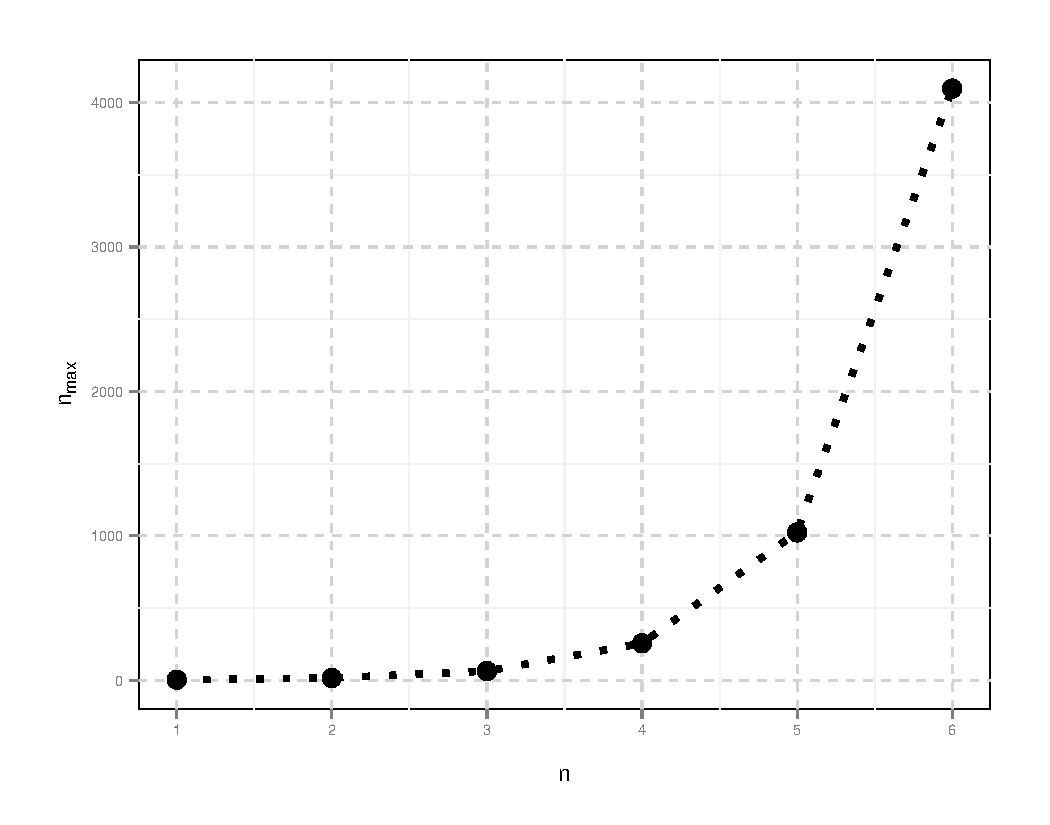
\includegraphics[width=\maxwidth]{figure/unnamed-chunk-5-1} 


\end{frame}

\subsection{Informacja o pozycji}

\begin{frame}

n-gramy mogą być przypisaną informację o pozycjach na których występują.

\end{frame}


\begin{frame}

% latex table generated in R 3.2.0 by xtable 1.7-4 package
% Wed May  6 09:37:40 2015
\begin{table}[ht]
\centering
\begin{tabular}{rllllll}
  \hline
 & P1 & P2 & P3 & P4 & P5 & P6 \\ 
  \hline
S1 & C & T & T & A & G & C \\ 
  S2 & C & A & G & A & C & G \\ 
  S3 & G & T & G & A & T & T \\ 
   \hline
\end{tabular}
\caption{Przykładowe sekwencje.  S - sekwencje, P - pozycja nukleotydu.} 
\end{table}

  

  
% latex table generated in R 3.2.0 by xtable 1.7-4 package
% Wed May  6 09:37:40 2015
\begin{table}[ht]
\centering
\begin{tabular}{rrrrrrrrr}
  \hline
 & 1\_A.A & 2\_A.A & 3\_A.A & 4\_A.A & 5\_A.A & 1\_C.A & 2\_C.A & 3\_C.A \\ 
  \hline
S1 & 0 & 0 & 0 & 0 & 0 & 0 & 0 & 0 \\ 
  S2 & 0 & 0 & 0 & 0 & 0 & 1 & 0 & 0 \\ 
  S3 & 0 & 0 & 0 & 0 & 0 & 0 & 0 & 0 \\ 
   \hline
\end{tabular}
\caption{Zliczenia 2-gramów z informacją o pozycji (fragment tabeli).} 
\end{table}


\end{frame}

\begin{frame}
$$n_\text{max} = p \times u^n$$

$n_\text{max}$: liczba wszystkich możliwych n-gramów

$p$: liczba możliwych pozycji.

$u$: liczba liter w alfabecie.

$n$: długość n-gramu

\end{frame}


\begin{frame}


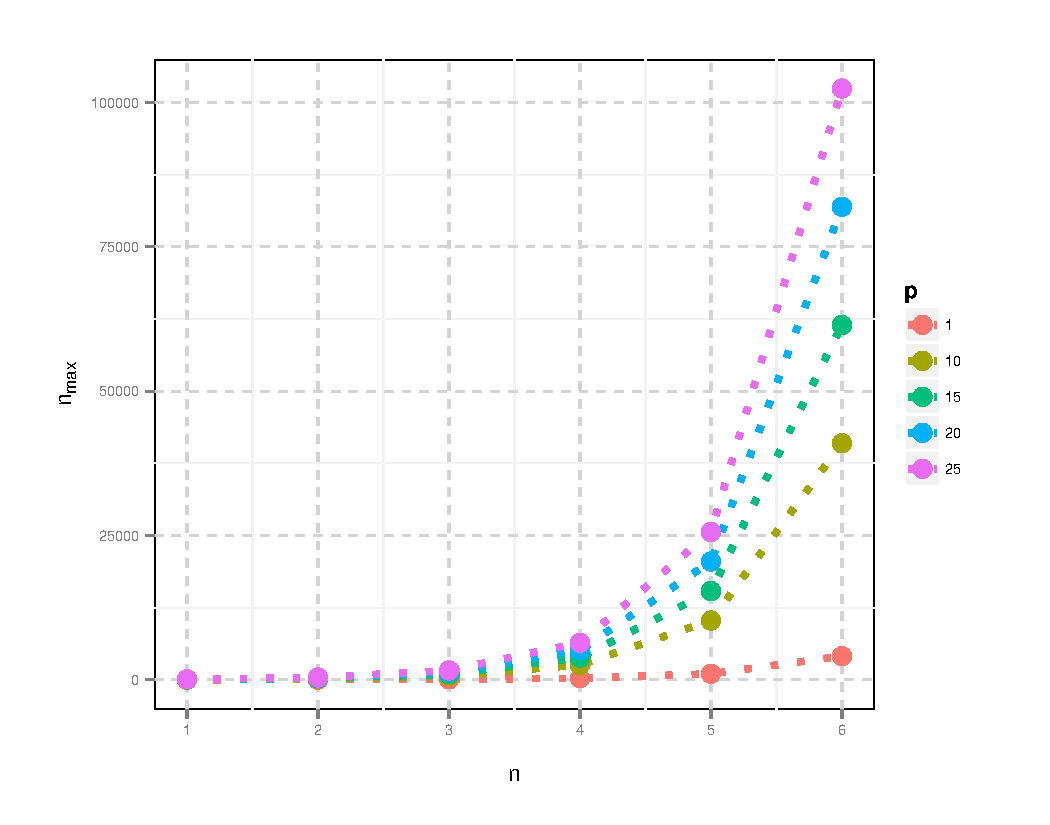
\includegraphics[width=\maxwidth]{figure/unnamed-chunk-8-1} 

\end{frame}

\subsection{Nieciągłe n-gramy}

\begin{frame}

n-gramy mogą być nieciągłe - pomiędzy elementami n-gramu mogą występować przerwy.

\end{frame}


\begin{frame}

% latex table generated in R 3.2.0 by xtable 1.7-4 package
% Wed May  6 09:37:41 2015
\begin{table}[ht]
\centering
\begin{tabular}{rllllll}
  \hline
 & P1 & P2 & P3 & P4 & P5 & P6 \\ 
  \hline
S1 & C & T & T & A & G & C \\ 
  S2 & C & A & G & A & C & G \\ 
  S3 & G & T & G & A & T & T \\ 
   \hline
\end{tabular}
\caption{Przykładowe sekwencje.  S - sekwencje, P - pozycja nukleotydu.} 
\end{table}

  

  
% latex table generated in R 3.2.0 by xtable 1.7-4 package
% Wed May  6 09:37:41 2015
\begin{table}[ht]
\centering
\begin{tabular}{rrrrrrrrr}
  \hline
 & A\_A & C\_A & G\_A & T\_A & A\_C & C\_C & G\_C & T\_C \\ 
  \hline
S1 & 0 & 0 & 0 & 1 & 1 & 0 & 0 & 0 \\ 
  S2 & 1 & 0 & 0 & 0 & 0 & 0 & 1 & 0 \\ 
  S3 & 0 & 0 & 0 & 1 & 0 & 0 & 0 & 0 \\ 
   \hline
\end{tabular}
\caption{Zliczenia 2-gramów z przerwą 1 (fragment tabeli).} 
\end{table}


\end{frame}

\subsection{Wybór informatywnych n-gramów - QuiPT}

\begin{frame}

Wielowymiarowa przestrzeń atrybutów jest filtrowana z pomocą QuiPT (\textbf{Qui}ck \textbf{P}ermutation \textbf{T}est) łączącego zalety testów permutacyjnych (brak założeń) z szybkością wykonania.

\end{frame}

\begin{frame}
W trakcie testu permutacyjnego oznaczenia klas są losowo mieszane na potrzeby obliczania statystyki testowej.
    
\begin{center}
\scalebox{0.85}{
$      
\textnormal{p-value} = \frac{N_{T_P > T_R}}{N}
$
}
\end{center}

gdzie $N_{T_P > T_R}$ to liczba losowań, kiedy $T_P$ (permutowana statystyka testowa) miała wartość krytyczniejszą niż $T_R$ (statystyka testowa dla niepermutowanych danych).
      
\end{frame}


\section{signalHSMM}

\subsection{Peptydy sygnałowe}

\begin{frame}

\begin{figure}[ht]
        \centering
        \scalebox{0.4}{
          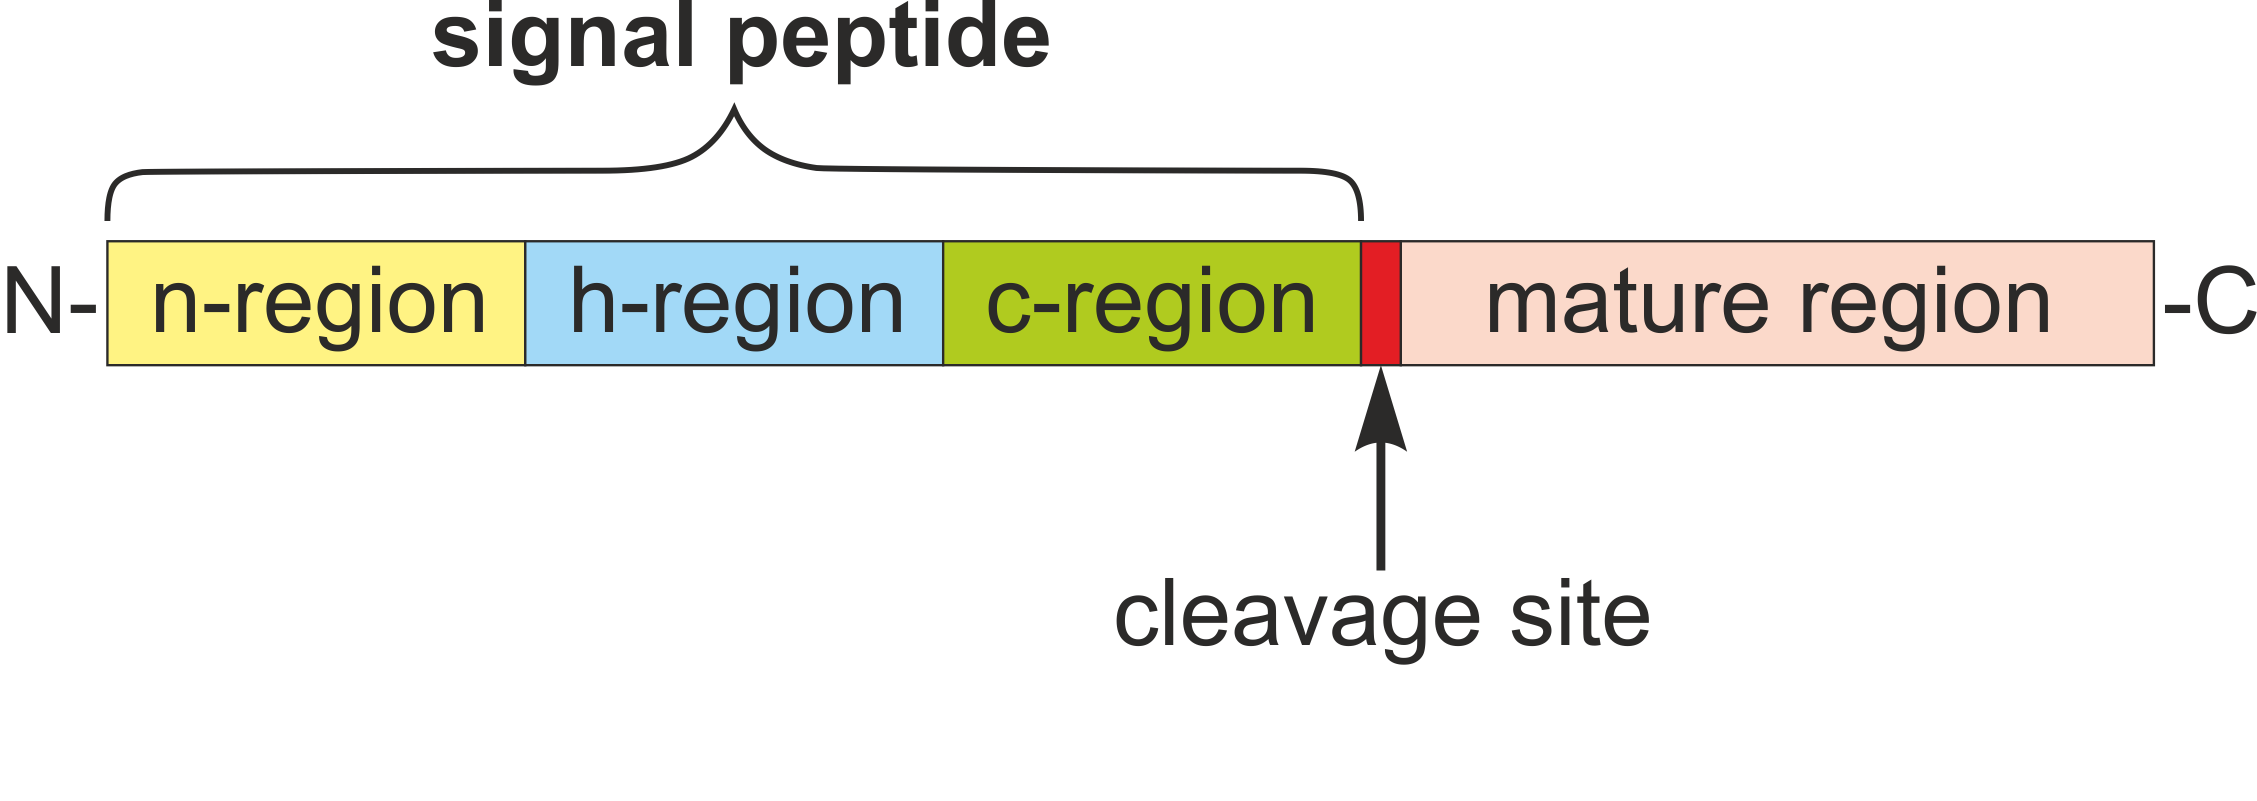
\includegraphics{SP.png}
        }
\end{figure}

      \begin{itemize}
        \item n-region: głównie zasadowe aminokwasy~\citep{nielsen_prediction_1998},
        \item h-region: silnie hydrofobowe reszty aminokwasy~\citep{nielsen_prediction_1998},
        \item c-region: kilka polarnych aminokwasów bez ładunku~\citep{jain_signal_1994}.
      \end{itemize}


\end{frame}

\begin{frame}

Istnieje szereg programów przewidujących występowanie peptydu sygnałowego:
\begin{itemize}
\item signalP 4.1 (sieci neuronowe)~\citep{petersen_signalp_2011},
\item PrediSi (Position Weight Matrix)~\citep{hiller_predisi:_2004},
\item Signal-3L (k-najbliszych sąsiadów)~\citep{shen_signal-3l:_2007},
\item Phobius (ukryte modele Markowa)~\citep{kall_combined_2004}.
\end{itemize}

\end{frame}

\subsection{Ukryte modele semi-Markowa}


\begin{frame}
      Założenia modelu:
      \begin{itemize}
        \item obserwowany rozkład aminokasów jest wynika z przebywania w określonym regionie (stanie),
        \item długość regionu (czas trwania stanu) jest modelowana poprzez rozkład prawdopodobieństwa (inny niż rozkład geometryczny jak w ukrytych modelach Markowa).
      \end{itemize}
    \end{frame}

    
    \begin{frame}
      \begin{enumerate}[1.]
        \item Pozyskanie eukariotycznych białek z bazy UniProtKB 2014\_07 (po ocyszczeniu z nietypowych lub niedokładnie opisanych rekordów zbiór danych liczy 3816 białek z peptydem sygnałowym i 9795 białek bez peptydu sygnałowego),
        \item określenie granic n-, h- i c-regionów przez algorytm heurystyczny,
        \item redukcja wymiarowości problemu poprzez zagregowanie aminokwasów na podstawie ich właściwości fizykochemicznych do kilku grup,
        \item obliczenie częstości występowania grup aminokwasowych w danych regionie oraz długości regionów,
        \item uczenie dwóch HSMM dla białek z peptydem sygnałowym i bez peptydu sygnałowego.
      \end{enumerate} 
    \end{frame}



\begin{frame}
    Podczas testowania, każde białko jest dopasowane do dwóch HSMM, które modelują odpowiednio białka bez peptydu sygnałowego i z peptydem sygnałowym. Prawdopodobieństwo obu dopasowań stanowią wynik działania programu.
    \begin{figure}
    \centering
    \resizebox{8.5cm}{!}{%
    \begin{tikzpicture}[->,>=stealth',shorten >=2pt,auto,node distance=4.5cm, thick]
      \tikzstyle{line} = [draw=black, color=blue!30!black!50, line width=4.5mm, -latex']
      \tikzstyle{main node} = [circle,fill=blue!20,draw, minimum size = 2.2cm, font=\itshape,
         align=center,  top color=white, bottom color=blue!50!black!70 ] %font=\sffamily\small\bfseries,
      %nodes
      \node[main node]            (start') 	[]						{Start};	     
      \node[main node, bottom color=purple!70!black!70] 	(nregion') 	[right of=start',xshift=-5mm, yshift=15mm] 	{n-region};
      \node[main node, bottom color=pink!70!black!70] 	(hregion') 	[right of=nregion',xshift=-5mm,yshift=15mm] 	{h-region};
      \node[main node, bottom color=gray!70!black!70] 	(cregion') 	[right of=hregion',xshift=-5mm,yshift=-15mm] 	{c-region};
      \node[main node, bottom color=green!70!black!70] 	(mature') 	[right of=cregion',xshift=-5mm, yshift=-15mm] 	{Mature protein};
      
      %lines
      \path [line] (start')   edge node [left, color=black] {} (nregion');
      \path [line] (nregion') edge node [below, color=black] { } (hregion');
      \path [line] (hregion') edge node [below, color=black] { } (cregion');
      \path [line] (cregion') edge node [left, color=black] { } (mature');
      \draw [line] (start') to[out=340,in=200] (mature');
    \end{tikzpicture} }
    \end{figure}


    \end{frame}




\begin{frame}

\tiny{
      \bibliographystyle{apalike}
      \bibliography{amyloid_present}
    }


\end{frame}

\end{document}
